\documentclass[]{article}
\usepackage{graphicx}
\usepackage[left=0.40in,top=0.2in,right=0.75in,bottom=0.2in]{geometry}
%opening
\title{Problem Set 8}
\author{Rodrigo Chavez Zavaleta}

\begin{document}

\maketitle

\section{Problem 1}
Please see problem1.pdf file.

\section{Problem 2}

a) Now we evaluate log(1/r) to find the potential everywhere but at the origin. Since we know the potential around the origin is the potential of its neighbours, we work out the potential at the origin as follows:
$$
	V[1,0] = (V[2,0] + V[0,0] + V[1,1] + V[1,-1])/4
$$
Rearranging, this yields:
$$
	V[0,0] = 4V[1,0] - (V[2,0] + V[1,1] + V[1,-1])
$$
Computing the asked values, we obtain the following:
\\
Potential at origin: 1.0\\
Density at origin: 1.0\\
Potential at [1, 0]: 0.0\\
Potential at [2, 0]: -0.5\\
Potential at [5, 0]: -1.1609640474436809\\

\begin{figure}[h!]
	\centering
	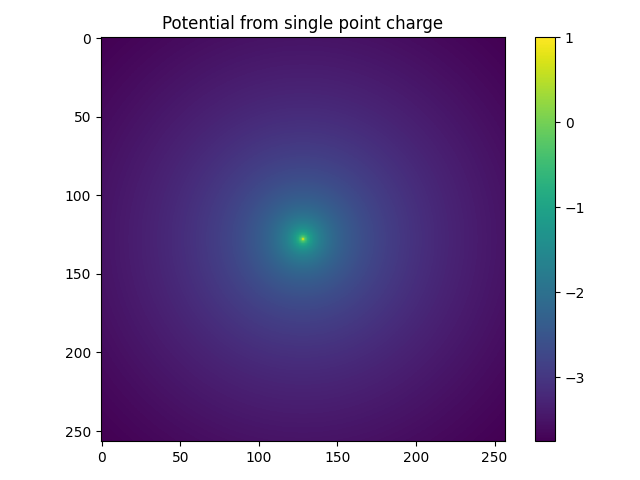
\includegraphics[width=0.5\linewidth]{../Results/2a1.png}
\end{figure}

\newpage
b) We now write a conjugate gradient solver to find the charge density on a square box held at V=1. here we present our results for the (absolute) charge density given the fixed potential.

\begin{figure}[h!]
	\centering
	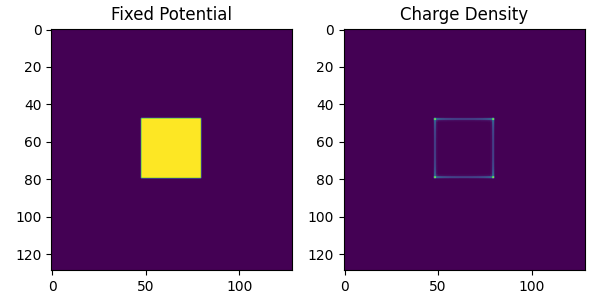
\includegraphics[width=0.75\linewidth]{../Results/2b1.png}
\end{figure}

And the charge density along one side

\begin{figure}[h!]
	\centering
	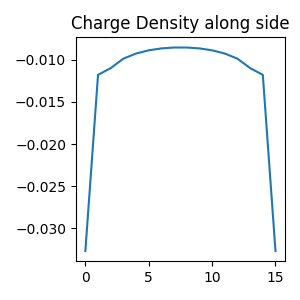
\includegraphics[width=0.25\linewidth]{../Results/2b2.png}
\end{figure}

We note that if we consider the square region to be a conductor, it makes physical sense to have a constant potential, Electric field zero inside the conductor, and the charge to lie on the boundary.

We verify our charge density solution by comparing the potential on the square obtained from convolving the density with the green's function, and we obtain an average absolute error in the order of $10^{-12}$.

\newpage

c)
Convolving our charge density found by conjugate gradient with the green's function, we find the potential everywhere and display it with equipotential lines in white.

\begin{figure}[h!]
	\centering
	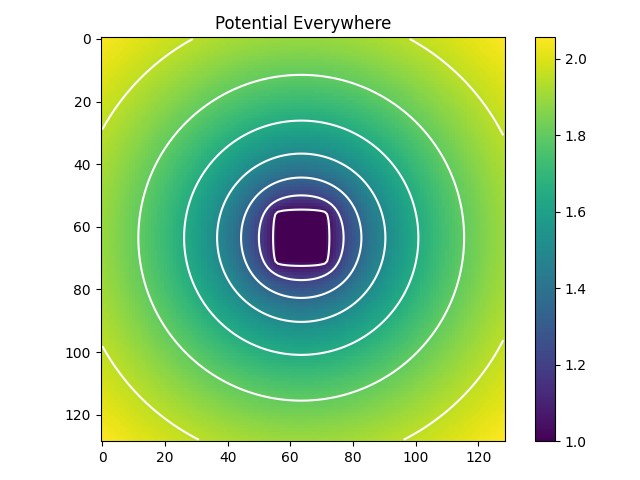
\includegraphics[width=0.5\linewidth]{../Results/2c1.png}
\end{figure}

To see how close to constant the potential is in the interior of the box, we compute the gradient of the potential and display its magnitude. 

\begin{figure}[h!]
	\centering
	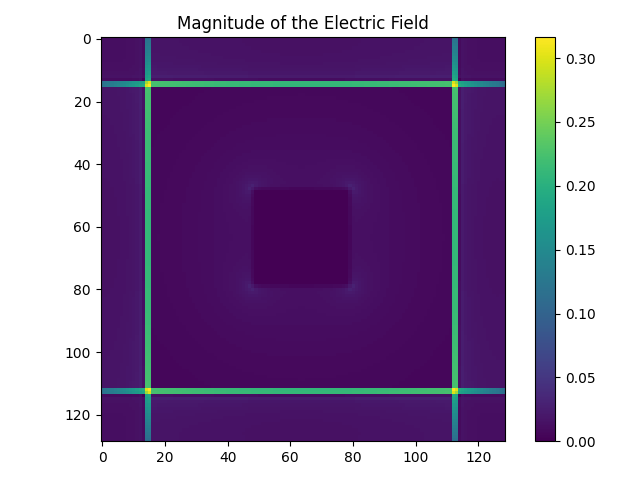
\includegraphics[width=0.45\linewidth]{../Results/2c2.png}
\end{figure}
Unsurprisingly, the magnitude of the electric field is larger for regions around larger charge density as found in b). Interpreting the electric field magnitude, we can say that the potential is close to constant towards the middle of the square.

We now look at the electric field line directions just outside of the box. As expected, The electric field lines are perpendicular to equipotential lines.

\begin{figure}[h!]
	\centering
	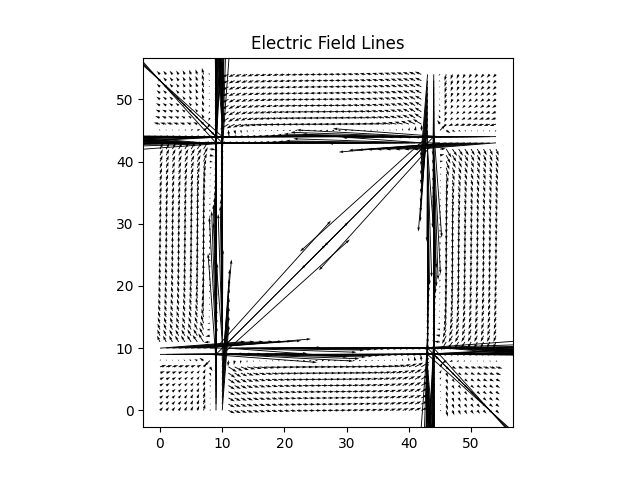
\includegraphics[width=0.45\linewidth]{../Results/2c3.png}
\end{figure}


\end{document}
